\documentclass[12pt,a4paper]{article}
\usepackage[utf8]{inputenc}
\usepackage[german]{babel}
\usepackage{amsmath}
\usepackage{amsfonts}
\usepackage{amssymb}
\usepackage{makeidx}
\usepackage{graphicx}
\usepackage{pdfpages}

\usepackage{fancyhdr}
\pagestyle{fancy}
\fancyhf{}

\usepackage{color}
%\usepackage[usenames,dvipsnames]{xcolor}
\usepackage{listings}
\lstset{numbers=left, numberstyle=\tiny, stepnumber=2, numbersep=5pt,frame=single}
\lstset{backgroundcolor=\color{yellow}}

\newcommand{\version}{1.0 }
\newcommand{\dateversion}{V\version (Dez12)}

\fancyhead[L]{\small{JP: RaspberryPi-MSRT}}

\fancyhead[C]{\small{Softwarebeschreibung}}
\fancyhead[R]{\thepage}


\renewcommand{\headrulewidth}{0.05pt}
\renewcommand{\footrulewidth}{0.05pt}

\author{Martin Seibl \and Fabian Hofmann}
\title{Raspberry Pi MSRT  \\ Software Dokumentation}

\fancyfoot[C]{\small{Martin Seibl, Fabian Hofmann}}
\fancyfoot[R]{\dateversion}
\fancyfoot[L]{
\includegraphics[scale=0.03]{logo/Raspberry_Pi_Logo.eps}}

\begin{document}
\begin{titlepage}
\maketitle

\begin{figure}[htp]
\centering
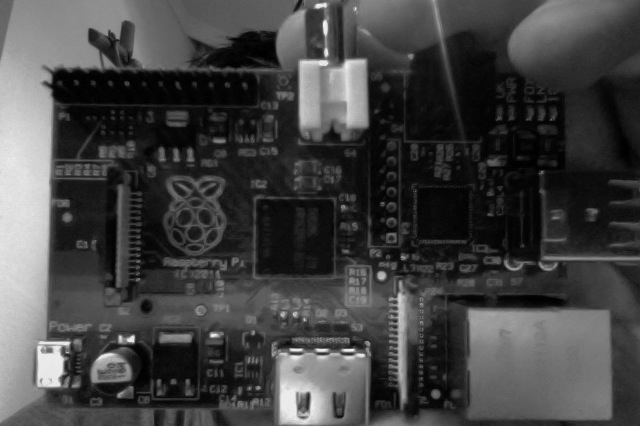
\includegraphics[width=0.9\textwidth]{pics/logo.jpg} 
\caption{Titelbild}
\end{figure}

\begin{center}
\large{Feinkonzept der IO Programmierung}\\
\large{Version \version}\\
\large{Klasse HN4Y}\\
\end{center}

\large{History:} \par
(V1.0) \textit{First Release}

\end{titlepage}

\tableofcontents

\newpage
\section{Aufgabenstellung}
Ein sich stetig erhitzender Kühlkörper soll mithilfe eines Lüfters gekühlt werden.  Die Temperatureinstellung wird mithilfe eines Webservers am Raspberry Pi realiesiert. Der Kühlkörper selbst wird mithilfe eines Transistors aufgeheitzt. Die Temperatur des Kühlkörpers soll mithilfe eines Sensors gemessen und in eine Datenbank gespeichert werden, um diese nachher Graphisch darzustellen. 
Die Steuerung des Lüfters geschieht mithilfe von einer softwareimplementeierten Variante von PWM, dazu werden Real Time Linux Komponenten verwendet. 

\begin{table}[htp]
\centering
\begin{tabular}{|c|c|}
\hline 
Autor & Zuständigkeitsbereich \\ 
\hline 
\hline
Martin Steibl & Hardwareentwicklung \\ 
\hline 
Fabian Hofmann & Sotwareentwicklung \\ 
\hline 
\end{tabular}
\caption{Aufgabenverteilung} 
\end{table}

\section{Beschreibung des Raspberry Pi}
\subsection{Allgemein}
Das Raspberry Pi (\textit{eng. raspberry = Himmbere, eng. pi = Kreiszahl}) is ein Embedded Computer. Ein Embedded Computer Computer der sehr klein und energiesparend konzipiert wurde. Es wurde von der \textit{ Raspberry Pi Foundation} entwickelt und hat Anwendungen (bedingt durch den HDMI Anschluss) als Multimediaplattform (XBMC, Sickbeard etc.) und als Schulungsplattform in den Einstieg in Embedded Computing Welt.

\subsection{Technische Specification}
\subsubsection{Der Prozessor}

\subsubsection{Interfaces}

\subsubsection{General Porpose IO - Pins}

\section{Vorbereitung der Plattform}
\subsection{Die SD-Karte vorbereiten}
Nun wird eine SD-Karte (SanDisk Ultra 16GB Class 10 30MB/s) in den SD-Kartenslot des Laptops eingeführt. Die SD-Karte wird erkannt. Nun haben wir die Wahl, welches Betriebssystem (OS,\textit{Operating System}) wir auf das Raspberry PI betreiben. Das jeweilige ISO-File befindet isch auf der www.raspberrypi.com/download. 

\subsubsection{Debian Linux}
\subsubsection{Arch Linux}

\begin{lstlisting}[caption={ISO-to-SD},label=iso,language = bash] 
fabian@fabian-ThinkPad-T430:~$ 
fabian@fabian-ThinkPad-T430:~$ 
fabian@fabian-ThinkPad-T430:~$ 
fabian@fabian-ThinkPad-T430:~$ 
fabian@fabian-ThinkPad-T430:~$ 
fabian@fabian-ThinkPad-T430:~$ 
fabian@fabian-ThinkPad-T430:~$ 
fabian@fabian-ThinkPad-T430:~$ 
\end{lstlisting}

\section{Programmablauf}
.
\begin{figure}[htp]
\centering
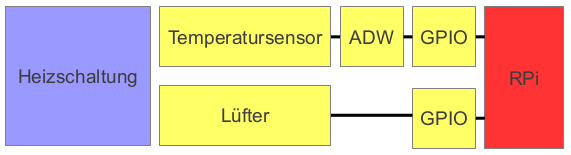
\includegraphics[width=0.9\textwidth]{pics/block.png} 
\caption{Blockschaltbild}
\end{figure}
.

\section{Ansteuerung mit $I^2C$}

\section{Ansteuerung mit PWM}


\appendix
\newpage
\section{Literatur- und Quellenverzeichnis}

\listoffigures
\listoftables

\section*{Autorenverzeichnis}
\section*{Literatur}

\newpage
\section{Datasheets}
\subsection{Datasheet for MCP3008}
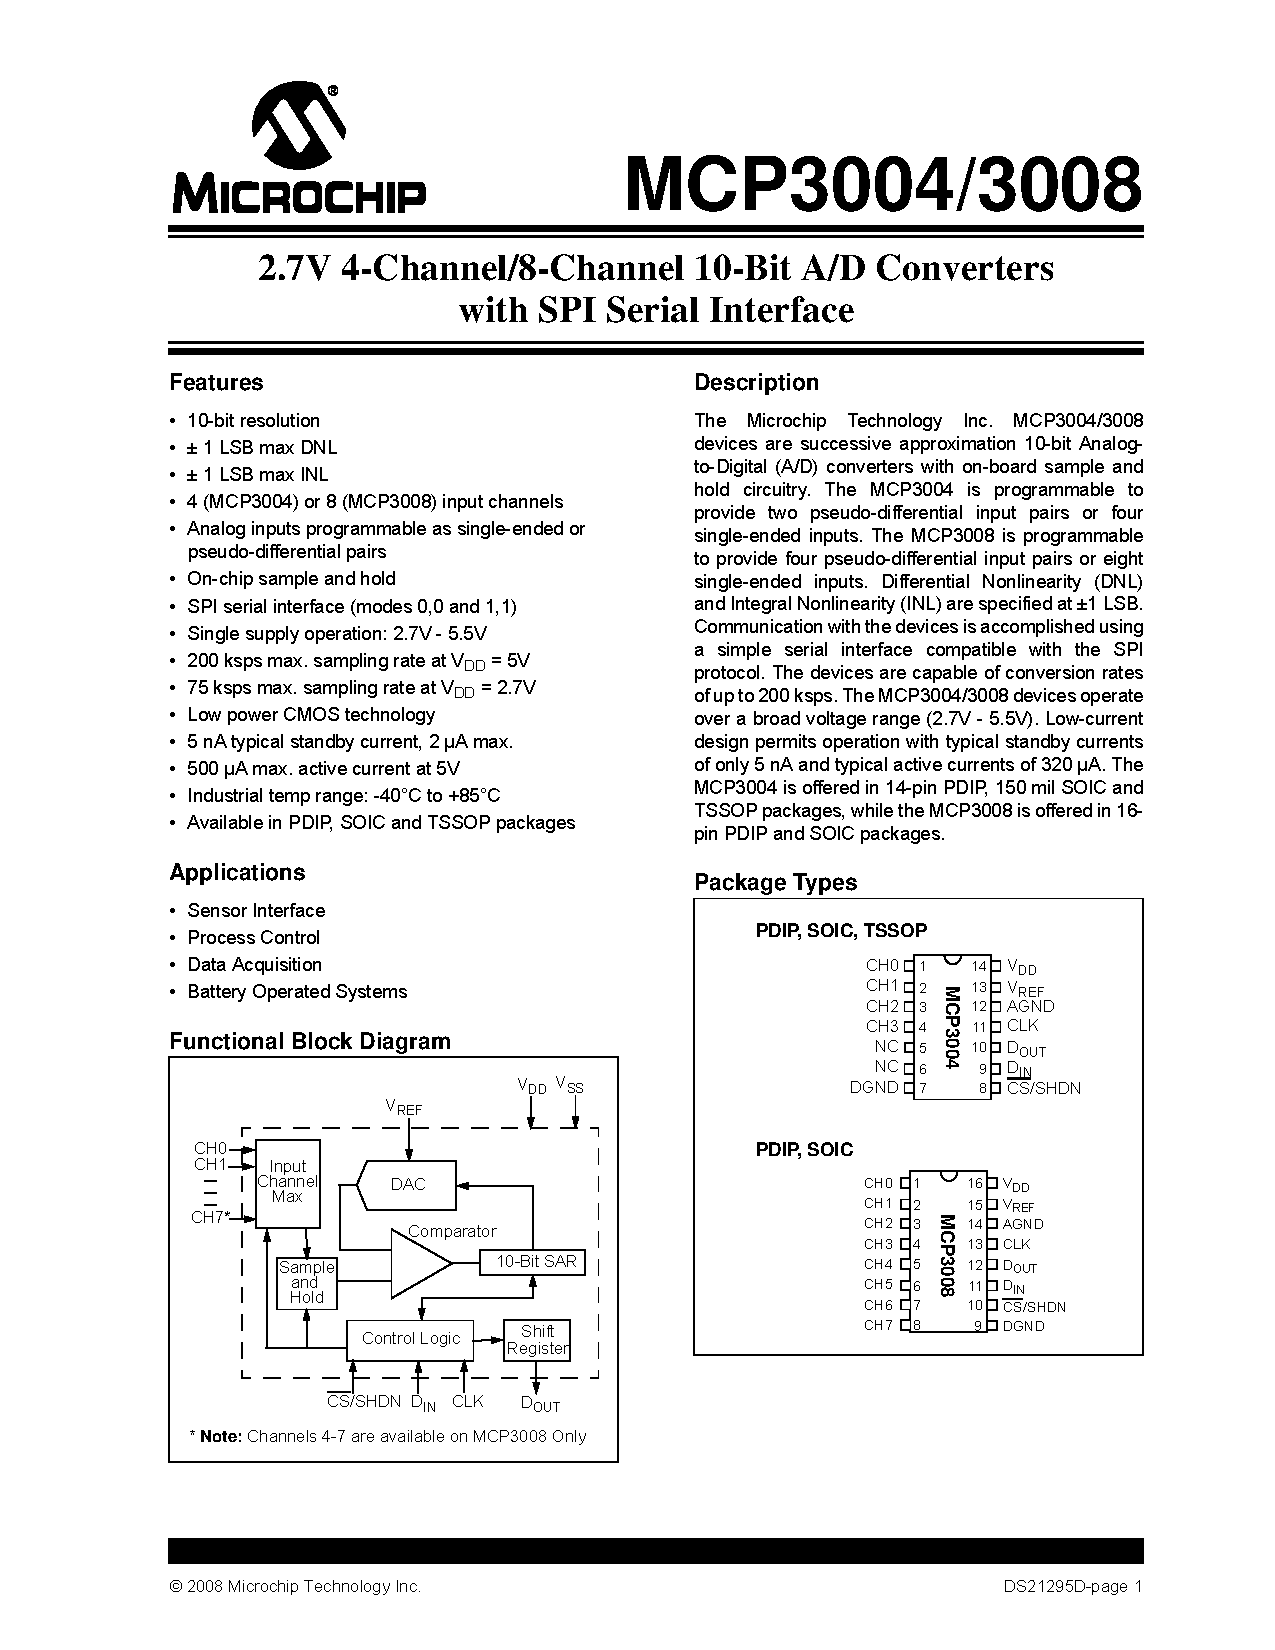
\includepdf[pages = 1]{datasheets/DS:MCP3008}
\includepdf[pages = 3-23]{datasheets/DS:MCP3008}

\end{document}